
\documentclass{article}
\usepackage{amsmath}
\usepackage{listings}
\usepackage{graphicx}
\usepackage[margin=1in]{geometry}
\pagenumbering{gobble}
\setlength{\tabcolsep}{10pt}
\renewcommand{\arraystretch}{1.7}
 
\begin{document}

\section*{\hfil C. Menutup Meriam\hfil}

% \begin{center}
% \begin{tabular}{ |cc| } 
%  \hline
%  Time Limit & 2 detik \\
%  \hline 
%  Memory Limit & 256 MB \\
%  \hline
% \end{tabular}
% \end{center}

\subsection*{Deskripsi}

\par\noindent Bocan sedang berperang melawan Turpa. Untuk memertahankan bentengnya, Bocan membuat $N$ buah meriam yang diletakkan pada sebuah garis lurus. Meriam tersebut diletakkan secara berjejer-jejer sehingga meriam ke-$i$ terletak pada petak ke-$i$. Setiap meriam memiliki tinggi masing-masing, meriam ke-$i$ memiliki tinggi $H_i$. Berikut adalah contoh $5$ buah meriam yang memiliki tinggi $3, 5, 2, 1, 3$ secara berturut-turut.

\begin{figure}[h!]
	\centering
	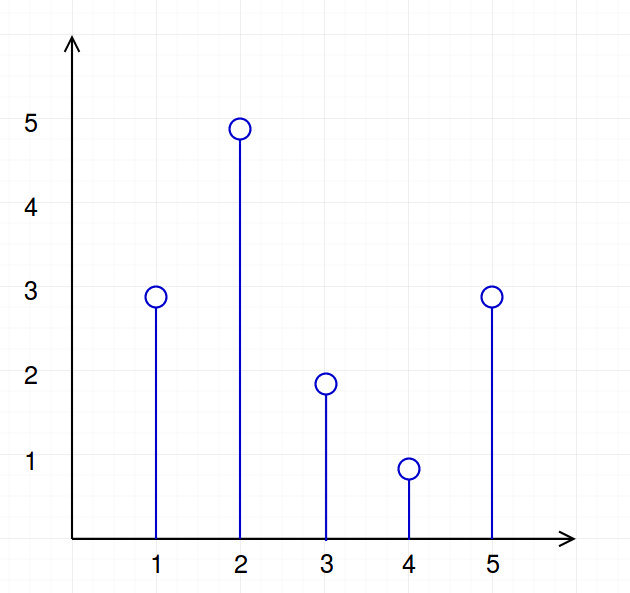
\includegraphics[width=0.2\linewidth]{meriam1.png}
	% \caption{Contoh Meriam 1}
\end{figure}

\par\noindent Karena tidak ingin meriamnya dilihat oleh Turpa, Bocan berusaha menutup meriamnya dengan terpal. Karena uang Bocan sudah habis untuk membuat meriam, Ia ingin agar terpal yang digunakan untuk menutup meriam sependek mungkin. Akan tetapi, meriam yang dimiliki Bocan sangat sensitif sehingga bila tersentuh sedikit saja bisa membuatnya menjadi rusak dan akurasinya berkurang. Oleh karena itu Bocan meminta bantuan Anda untuk menjawah $Q$ buah pertanyaan. Setiap pertanyaan, Bocan akan
memberikan dua buah bilangan yaitu $L$ dan $R$ kemudian menanyakan berapa banyak meriam yang akan rusak jika ia menutup meriam ke-$L$ hingga $R$ (meriam ke-$i$ dimana $L \leq i \leq R$) dengan terpal sependek mungkin.

\par\noindent Proses penutupan terpal pada meriam dilakukan dengan memasang terpal pada ujung-ujung meriam. Gambar dibawah ini menunjukkan cara penutupan meriam ke-$2$ hingga $5$.

\begin{figure}[h!]
	\centering
	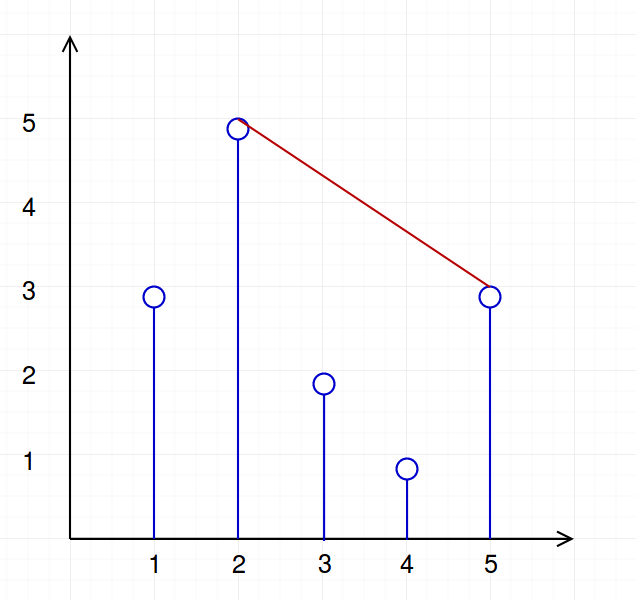
\includegraphics[width=0.2\linewidth]{meriam2.png}
	% \caption{Contoh Penutupan Meriam}
\end{figure}

\subsection*{Format Masukan}

\par\noindent Baris pertama dari input berisi sebuah bilangan bulat $N$ yang menyatakan banyaknya meriam yang dimiliki bocan.
\par\noindent Baris kedua berisi $N$ buah bilangan bulat. Bilangan ke-$i$ menyatakan nilai $H_i$ yaitu tinggi meriam ke-$i$.
\par\noindent Baris ketiga berisi sebuah bilangan bulat $Q$ yang menyatakan banyaknya pertanyaan yang diajukan Bocan.
\par\noindent $Q$ baris berikutnya berisi dua buah bilangan bulat $L$ dan $R$ seperti yang dijelaskan pada deskripsi soal.

\subsection*{Format Keluaran}

\par\noindent Output berisi $Q$ baris dimana setiap baris ke-$i$ berisi sebuah bilangan bulat yang merupakan jawaban dari pertanyaan Bocan yang ke-$i$.

\subsection*{Contoh Masukan}

\begin{lstlisting}
7
4 1 2 3 2 3 1
2
2 5
1 7
\end{lstlisting}

\subsection*{Contoh Keluaran}

\begin{lstlisting}
4
3
\end{lstlisting}

\subsection*{Penjelasan}

\par\noindent Meriam pada contoh tersebut dapat digambarkan seperti berikut:

\begin{figure}[h!]
	\centering
	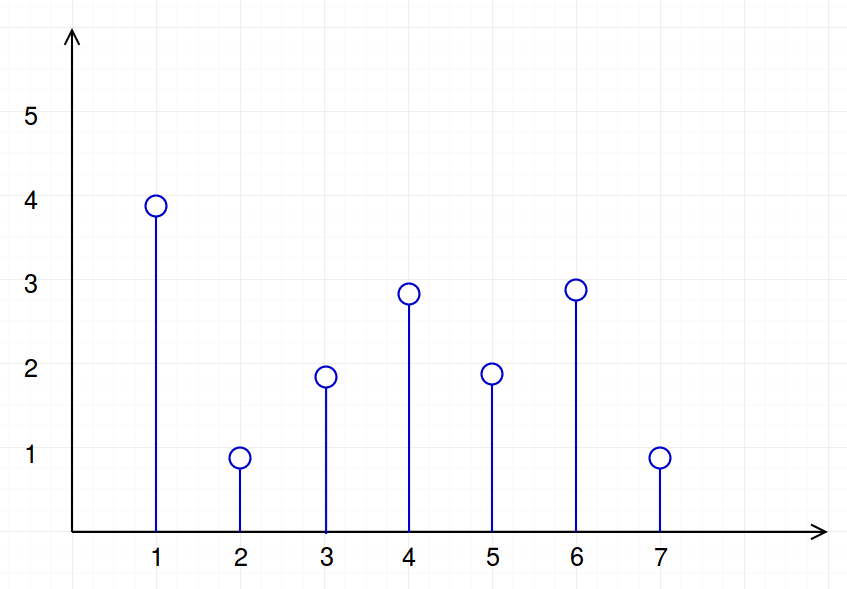
\includegraphics[width=0.4\linewidth]{meriam_sample1.png}
	% \caption{Konfigurasi Meriam Pada Contoh}
\end{figure}

\par\noindent Untuk pertanyaan pertama, meriam ke-dua, tiga, empat dan lima akan terkena terpal.
\par\noindent Sedangkan untuk pertanyaan ke-dua, meriam pertama ke-enam dan ke-tujuh akan terkena terpal.
\par\noindent Perhatikan gambar berikut:

\begin{figure}[h!]
	\centering
	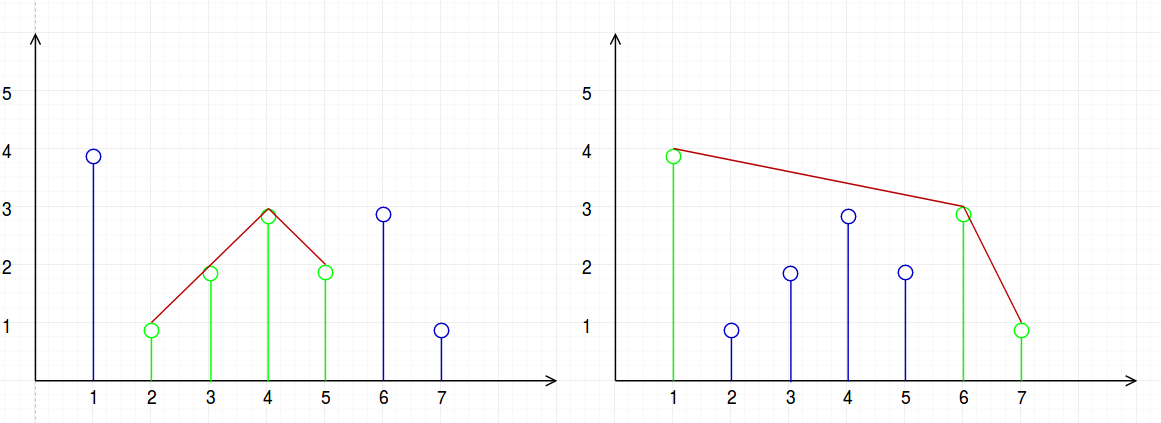
\includegraphics[width=0.7\linewidth]{meriam_sample2.png}
	% \caption{Penutupan Meriam}
\end{figure}

\subsection*{Batasan}

\begin{itemize}
	\item $1 \leq N, Q \leq 50000$
	\item $1 \leq H_i \leq 50000$
	\item $1 \leq L_i < R_i \leq N$
\end{itemize}

\end{document}
